\documentclass[conference]{IEEEtran}
\IEEEoverridecommandlockouts

\usepackage{cite}
\usepackage{amsmath,amssymb}
\usepackage{graphicx}
\usepackage{booktabs}
\usepackage{array}
\usepackage{multirow}
\usepackage{xcolor}
\usepackage{listings}
\usepackage{tikz}
\usetikzlibrary{positioning,arrows.meta,fit,calc}
\usepackage[hidelinks]{hyperref}
\usepackage{url}

\newcommand{\benchSpeedupMin}{225}
\newcommand{\benchSpeedupMax}{878}
\newcommand{\benchOverheadMin}{29}
\newcommand{\benchOverheadMax}{217}
\newcommand{\benchCPU}{Intel Xeon Processor @ 2.10GHz}
\newcommand{\benchCC}{13.3.0}
\newcommand{\benchPython}{3.13.16}
\newcommand{\benchAllMatch}{all outputs matched}

% Primitive \input, so generated table rows can be read inside a tabular
\makeatletter
\newcommand{\inputrows}[1]{\@@input #1 }
\makeatother

% ---------------------------------------------------------------- listings
\definecolor{kw}{HTML}{1F3A93}
\definecolor{ty}{HTML}{6A2C91}
\definecolor{cm}{HTML}{5F6368}
\definecolor{st}{HTML}{1B6B3A}
\lstdefinelanguage{cmm}{
  morekeywords={module,fn,main,let,mut,if,else,while,do,for,print,true,false,return,switch,case,default},
  morekeywords=[2]{int,float,bool,string,array,list,stack,queue},
  sensitive=true,
  morecomment=[l]{//},
  morecomment=[s]{/*}{*/},
  morestring=[b]",
}
\lstset{
  basicstyle=\ttfamily\footnotesize,
  keywordstyle=\color{kw}\bfseries,
  keywordstyle=[2]\color{ty},
  commentstyle=\color{cm}\itshape,
  stringstyle=\color{st},
  columns=fullflexible,
  keepspaces=true,
  frame=lines,
  framesep=3pt,
  xleftmargin=3pt,
  xrightmargin=3pt,
  aboveskip=6pt,
  belowskip=4pt,
  captionpos=b,
  showstringspaces=false,
  literate={--}{{-{}-}}2,
}
\lstdefinestyle{diag}{language={},basicstyle=\ttfamily\fontsize{6.6}{7.6}\selectfont,keywordstyle={},literate={},
  breaklines=true,breakatwhitespace=true,postbreak=\mbox{\hspace{1.2em}}}

\newcommand{\cmm}{C\texttt{-{}-}}

\begin{document}

\title{\cmm{} (C Minus Minus): A Statically Checked\\Imperative Language Achieving Memory Safety by Removal}

\author{
\IEEEauthorblockN{Ronit Mexson}
\IEEEauthorblockA{\textit{School of Computer Science and}\\
\textit{Engineering (SCOPE)}\\
Reg.\ No.\ 24BAI0036}
\and
\IEEEauthorblockN{Mit Kumar Raju Panchal}
\IEEEauthorblockA{\textit{School of Computer Science and}\\
\textit{Engineering (SCOPE)}\\
Reg.\ No.\ 24BAI0279}
\and
\IEEEauthorblockN{Garv Gupta}
\IEEEauthorblockA{\textit{School of Computer Science and}\\
\textit{Engineering (SCOPE)}\\
Reg.\ No.\ 24BDS0169}
}

\maketitle

\begin{abstract}
Memory-safety defects remain the dominant source of severe vulnerabilities in software written in C and C++.
Existing remedies either add machinery to the language (garbage collection, ownership and borrow checking,
fat pointers) or detect faults after the fact (sanitizers). This paper presents \cmm{} (C Minus Minus), a small,
statically typed, C-like imperative language built on the opposite principle, \emph{safety by removal}: the
constructs that make memory corruption and undefined behaviour expressible are deleted from the grammar
instead of being guarded. \cmm{} has no pointers, no null, no uninitialized variables, no implicit conversions
and no undefined behaviour; bindings are immutable by default; collections have deep-copy value semantics;
and every remaining fault (integer overflow, division by zero, out-of-range indexing, unbounded recursion)
is a deterministic, positioned runtime trap. We describe the language, its zero-dependency Python
implementation (lexer, recursive-descent parser, semantic analyzer, reference interpreter and ISO~C99
transpiler), a diagnostics system with 60 documented error codes written for novices, and a browser-based
compiler studio. The evaluation maps eleven common weakness classes to the mechanism that eliminates or traps
them, reports a 445-test suite (444 passing, with the remaining failure analysed), and measures the
transpiled C99 against both the interpreter and hand-written unchecked C.
\end{abstract}

\begin{IEEEkeywords}
programming languages, memory safety, compilers, static analysis, language design, transpilation, compiler diagnostics
\end{IEEEkeywords}

% ======================================================================
\section{Introduction}
% ======================================================================
For decades, systems software has been written in C and C++, languages whose flexibility comes from raw
pointers, manual memory management and a large catalogue of undefined behaviour. The cost is well documented:
Microsoft has reported that roughly 70\% of the vulnerabilities it assigns a CVE each year are memory-safety
issues~\cite{miller2019}, the Chromium project reports a similar share among its serious security
bugs~\cite{chromium_memsafety}, and government agencies now urge vendors to publish memory-safety
roadmaps~\cite{cisa2023}.

Two families of remedies dominate. \emph{Additive} approaches extend the language with new machinery:
safe dialects such as Cyclone~\cite{cyclone}, CCured~\cite{ccured} and Checked~C~\cite{checkedc} add
annotated pointer kinds and runtime metadata, while Rust~\cite{rust} adds ownership, borrowing and
lifetimes. \emph{Detective} approaches such as AddressSanitizer~\cite{asan} keep the language unchanged
and find faults during testing. Both are effective, but the first raises the conceptual burden on
programmers and the second offers no guarantee in production.

This paper explores a third option for the setting of education and small, high-assurance programs:
\emph{safety by removal}. Instead of adding mechanisms that make dangerous features safe, \cmm{} removes the
dangerous features and keeps only constructs whose behaviour is fully specified. The guiding question is how
much of C's explicit, predictable programming style survives when every construct with undefined behaviour
is taken away. The contributions are:
\begin{itemize}
  \item the design of \cmm{}, a statically typed imperative language without pointers, null, uninitialized
        state, implicit conversions or undefined behaviour, with immutable-by-default bindings and
        deep-copy value semantics for collections (Section~\ref{sec:design});
  \item a complete, dependency-free implementation with two execution back ends: a normative tree-walking
        interpreter and an ISO~C99~\cite{iso_c99} transpiler with checked arithmetic (Section~\ref{sec:impl});
  \item a diagnostics system of 60 documented error codes that explains each error in plain language and
        proposes a concrete fix (Section~\ref{sec:diag});
  \item an evaluation of the safety guarantees, test coverage and performance cost of the approach
        (Section~\ref{sec:eval}).
\end{itemize}

The name follows the language's philosophy, \emph{C minus the dangerous parts}. It is unrelated to the
portable assembly language of the same name used inside the Glasgow Haskell Compiler~\cite{cmm_ghc}.

% ======================================================================
\section{Related Work}
% ======================================================================
\textbf{Safe C dialects.} Cyclone~\cite{cyclone} restricts pointer arithmetic, adds region-based memory
management and several pointer kinds. CCured~\cite{ccured} infers pointer kinds and inserts run-time checks
for legacy code, and Checked~C~\cite{checkedc} adds checked pointer and array types that can be adopted
incrementally. These systems retain pointers and therefore must track them; \cmm{} removes them.

\textbf{Ownership-based languages.} Rust~\cite{rust} achieves memory safety without garbage collection through
ownership and borrowing, at the price of lifetime reasoning that is notoriously hard for beginners. \cmm{}
obtains alias freedom more crudely but far more simply: every collection is a value, copied on assignment and
argument passing.

\textbf{Subsets and verification.} MISRA~C~\cite{misra} restricts C through coding rules enforced by external
checkers, and SPARK~\cite{spark} restricts Ada so that programs can be formally verified. \cmm{} shares their
subsetting philosophy but enforces the restrictions in the grammar and type system of a standalone language,
so that a violating program cannot be written at all.

\textbf{Error messages.} Research on novice programmers shows that terse compiler messages are a major
obstacle~\cite{becker2019}, and languages such as Elm popularized messages written for
humans~\cite{elm_errors}. \cmm{} adopts this style for every one of its diagnostics.

% ======================================================================
\section{Language Design}\label{sec:design}
% ======================================================================
\subsection{Principles}
Three rules govern every design decision. \emph{(i) Remove rather than guard:} a feature whose misuse causes a
vulnerability class is omitted unless it can be given fully defined semantics. \emph{(ii) No undefined
behaviour:} every program either has a precisely specified result or stops with a precisely specified,
positioned error. \emph{(iii) Explicitness over convenience:} there are no implicit narrowing conversions, no
truthiness and no operators whose meaning depends on context.

\subsection{Types and values}
\cmm{} has four primitive types and four generic collection types (Table~\ref{tab:types}). Integers are 64-bit
two's-complement values whose every operation is range-checked; division and remainder truncate toward zero,
so the identity $(a/b)\cdot b + a \bmod b = a$ holds for all non-zero divisors. Floats follow IEEE~754
binary64~\cite{ieee754}, but infinities and NaN can never be produced: an overflow or a division by zero is a
runtime error instead. The only implicit conversion is the widening of an \texttt{int} operand to
\texttt{float} in mixed arithmetic and comparison; assignment never converts.

\begin{table}[t]
\caption{Types of \cmm{} v0.2.0}
\label{tab:types}
\centering
\footnotesize
\begin{tabular}{@{}l p{5.3cm}@{}}
\toprule
\textbf{Type} & \textbf{Semantics} \\
\midrule
\texttt{int}    & 64-bit signed; overflow traps (R001) \\
\texttt{float}  & IEEE~754 binary64; never Inf or NaN (R002, R004) \\
\texttt{bool}   & \texttt{true}/\texttt{false}; never converted to or from numbers \\
\texttt{string} & immutable Unicode text; indexing by code point, \texttt{.len()} \\
\midrule
\texttt{array<T>} & fixed length, bounds-checked indexing (R006) \\
\texttt{list<T>}  & growable; \texttt{push}, \texttt{pop}, \texttt{insert}, \texttt{remove}, \texttt{contains} \\
\texttt{stack<T>} & LIFO; \texttt{push}, \texttt{pop}, \texttt{peek}; empty pop traps (R012) \\
\texttt{queue<T>} & FIFO; \texttt{enqueue}, \texttt{dequeue}, \texttt{peek} \\
\bottomrule
\end{tabular}
\end{table}

\subsection{Bindings and mutability}
A variable is introduced with \texttt{let} (immutable) or \texttt{mut} (mutable) and \emph{must} be
initialized; the grammar has no declaration without an initializer, so an uninitialized read cannot be
written. Types are inferred from the initializer. Immutability is deep: on a \texttt{let} collection neither
element assignment (E029) nor mutating methods (E028) are allowed. Function parameters are immutable.

\subsection{Statements and control flow}
Assignment is a statement, not an expression, so \texttt{if (x = 1)} and \texttt{a = b = 0} are syntax
errors. The operators \texttt{++}, \texttt{--}, single \texttt{\&} and single \texttt{|} are rejected by the
lexer with a hint to use \texttt{+= 1}, \texttt{-= 1}, \texttt{\&\&} and \texttt{||}. Braces are mandatory
for every body, which removes the dangling-\texttt{else} problem. Conditions must have type \texttt{bool}.
A \texttt{switch} matches \texttt{int} or \texttt{string} literals, has no fall-through and rejects
duplicate cases at compile time.

\subsection{Functions}
Functions have typed parameters and an optional return type. The analyzer collects all signatures before
checking bodies, so definition order is free and mutual recursion works. A conservative
\emph{definitely-returns} rule rejects any typed function with a path that falls off the end (E013): a block
returns if any statement in it returns, an \texttt{if} only if it has an \texttt{else} and all branches
return, and loops never count. There are no globals; a function sees only its parameters. Recursion depth is
bounded at 1000 calls (R007) on every platform.

\subsection{Collections and value semantics}
Collections never alias. Assigning, passing or returning a collection copies it, so a callee can never
modify its caller's data and two names never observe each other's updates (Listing~\ref{lst:value}). This
removes the aliasing that ownership systems must otherwise track, at the cost of copying, which we accept in
exchange for a much simpler mental model.

\lstinputlisting[language=cmm,caption={Typed functions, a growable list and deep-copy value semantics.},label={lst:value},float=t]{examples/value_semantics.cmm}

Table~\ref{tab:hazards} summarizes how each language rule maps to the weakness class it removes.

% ======================================================================
\section{Implementation}\label{sec:impl}
% ======================================================================
The reference implementation is about 6\,300 lines of Python using only the standard library, so it runs
unchanged on Windows, macOS and Linux. Fig.~\ref{fig:pipeline} shows its structure.

\begin{figure}[t]
\centering
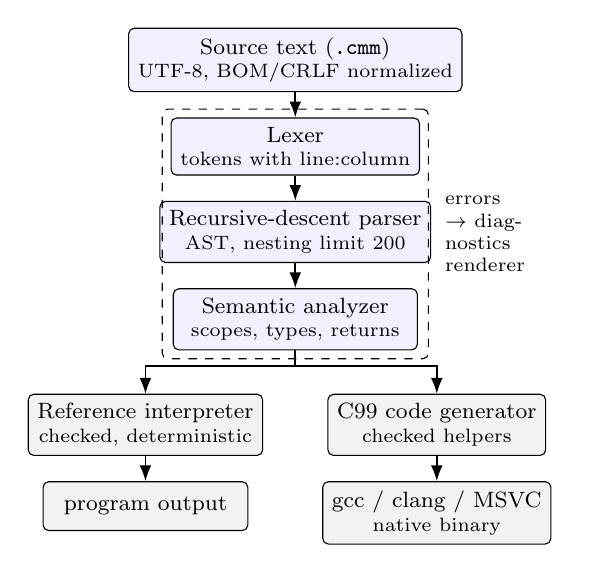
\begin{tikzpicture}[
  font=\footnotesize,
  cmmstage/.style={draw, rounded corners=2pt, fill=blue!6, minimum width=3.1cm, minimum height=0.62cm, align=center},
  cmmout/.style={draw, rounded corners=2pt, fill=gray!10, minimum width=2.6cm, minimum height=0.62cm, align=center},
  arr/.style={-{Latex[length=2mm]}, semithick},
  node distance=0.32cm]
  \node[cmmstage] (src) {Source text (\texttt{.cmm})\\[-1pt]\scriptsize UTF-8, BOM/CRLF normalized};
  \node[cmmstage, below=of src] (lex) {Lexer\\[-1pt]\scriptsize tokens with line:column};
  \node[cmmstage, below=of lex] (par) {Recursive-descent parser\\[-1pt]\scriptsize AST, nesting limit 200};
  \node[cmmstage, below=of par] (ana) {Semantic analyzer\\[-1pt]\scriptsize scopes, types, returns};
  \node[cmmout, below left=0.55cm and -1.15cm of ana] (int) {Reference interpreter\\[-1pt]\scriptsize checked, deterministic};
  \node[cmmout, below right=0.55cm and -1.15cm of ana] (cg) {C99 code generator\\[-1pt]\scriptsize checked helpers};
  \node[cmmout, below=of cg] (cc) {gcc / clang / MSVC\\[-1pt]\scriptsize native binary};
  \node[cmmout, below=of int] (stdout) {program output};
  \draw[arr] (src) -- (lex);
  \draw[arr] (lex) -- (par);
  \draw[arr] (par) -- (ana);
  \draw[arr] (ana.south) -- ++(0,-0.2) -| (int.north);
  \draw[arr] (ana.south) -- ++(0,-0.2) -| (cg.north);
  \draw[arr] (cg) -- (cc);
  \draw[arr] (int) -- (stdout);
  \node[draw, dashed, rounded corners=2pt, fit=(lex)(ana), inner sep=3pt] (fe) {};
  \node[right=0.08cm of fe, align=left, font=\scriptsize, text width=1.35cm] {errors\\$\rightarrow$ diagnostics renderer};
\end{tikzpicture}
\caption{Compilation pipeline. Each stage reports positioned errors to a shared diagnostics renderer.}
\label{fig:pipeline}
\end{figure}

\subsection{Front end}
The source is decoded as strict UTF-8; a byte-order mark is removed and line endings are normalized before
lexing, and columns count Unicode code points, so positions are identical on every platform. The
hand-written lexer uses longest-match tokenization and stops at the first lexical error. The parser is a
stratified recursive-descent parser~\cite{dragonbook} with one procedure per precedence level (logical or,
logical and, equality, comparison, additive, multiplicative, prefix and postfix), giving C's usual
precedence and left associativity. A nesting limit of 200 levels (S004) bounds recursion on adversarial
input.

\subsection{Semantic analysis}
The analyzer performs two passes: it first records every function signature, then checks each body with a
stack of lexical scopes. It resolves names, infers and checks types, enforces \texttt{let}/\texttt{mut}
rules, validates calls and method calls against a table of built-in collection methods, rejects duplicate
\texttt{switch} cases and applies the definitely-returns rule. All semantic errors in a program are
collected and reported in source order, rather than only the first one.

\subsection{Reference interpreter}
The normative semantics are given by a tree-walking interpreter. Every integer operation is checked against
$[-2^{63}, 2^{63}-1]$ and every float result against overflow; division by zero traps for both types.
Collections are copied on assignment and argument passing. Each call creates a fresh environment holding only
its parameters. To make the 1000-call depth limit behave identically on all platforms, the interpreter runs
in a thread with a 256\,MB stack. An optional step budget (\texttt{--max-steps}) bounds runaway loops, and the
web server uses it for untrusted code.

\subsection{ISO C99 back end}
The transpiler lowers the v0.1 subset plus user-defined functions to portable C99 that uses only standard
headers. Arithmetic is emitted as calls to small \texttt{static} helpers that perform the same overflow and
division checks as the interpreter, and a custom formatter reproduces the interpreter's shortest
round-trip float printing, so a transpiled program prints exactly what the interpreter prints. Collections,
indexing and \texttt{switch} are not yet supported by this back end; such programs are rejected with error
T001 rather than being compiled incorrectly.

\begin{table}[t]
\caption{Size of the reference implementation}
\label{tab:loc}
\centering
\footnotesize
\begin{tabular}{@{}l r@{}}
\toprule
\textbf{Component (modules)} & \textbf{Lines} \\
\midrule
Lexer and token definitions (\texttt{lexer}, \texttt{tokens}) & 585 \\
Parser and AST (\texttt{parser}, \texttt{ast\_nodes}) & 1\,343 \\
Semantic analyzer and type rules (\texttt{analyzer}, \texttt{types}) & 778 \\
Interpreter and runtime (\texttt{interpreter}, \texttt{runtime\_*}, \texttt{builtins}) & 1\,117 \\
C99 code generator (\texttt{codegen\_c}) & 859 \\
Diagnostics (\texttt{errors}, \texttt{explanations}, \texttt{suggest}, \texttt{diagnostic\_render}) & 867 \\
CLI and printers (\texttt{cli}, \texttt{astprint}, \texttt{formatting}, others) & 755 \\
\midrule
\textbf{Total} & \textbf{6\,304} \\
\bottomrule
\end{tabular}
\end{table}

\subsection{Tooling}
A command-line tool provides \texttt{run}, \texttt{check}, \texttt{tokens}, \texttt{ast} and
\texttt{transpile} commands with distinct exit codes for static errors, runtime traps and I/O failures.
A zero-dependency web studio exposes the same pipeline through a JSON API and a browser editor with syntax
highlighting, live diagnostics as the user types, and inspectors for tokens, the AST and the generated C99.

% ======================================================================
\section{Diagnostics}\label{sec:diag}
% ======================================================================
Because \cmm{} targets learners as well as careful programmers, every error is designed to be read by a
novice~\cite{becker2019}. Each of the 60 diagnostic codes (Table~\ref{tab:codes}) has a positioned headline,
a source excerpt with a caret under the offending token, a plain-language explanation under
\emph{what went wrong}, and a concrete repair under \emph{how to fix}, often with corrected code. For an
undeclared name, the analyzer proposes the closest declared identifier by Damerau--Levenshtein
distance~\cite{damerau,levenshtein}, accepting at most one edit for names shorter than five characters and two
otherwise (Listing~\ref{lst:diag}). A \texttt{--no-help} flag restores a terse
three-line format for tools.

\begin{table}[t]
\caption{Diagnostic codes by phase}
\label{tab:codes}
\centering
\footnotesize
\begin{tabular}{@{}l l r >{\raggedright\arraybackslash}p{3.85cm}@{}}
\toprule
\textbf{Prefix} & \textbf{Phase} & \textbf{Codes} & \textbf{Examples} \\
\midrule
L & Lexical      & 12 & \texttt{++} not supported, unterminated string \\
S & Syntax       & 3  & expected token, reserved word, nesting \\
E & Semantic     & 30 & undeclared name, \texttt{let} reassigned, missing return \\
R & Runtime      & 14 & overflow, division by zero, index range \\
T & Transpile    & 1  & feature not supported by the C back end \\
\midrule
  & \textbf{Total} & \textbf{60} & \\
\bottomrule
\end{tabular}
\end{table}

\lstinputlisting[style=diag,caption={Diagnostic for a misspelled identifier, as printed by \texttt{cmm run}.},label={lst:diag},float=t]{generated/diag_typo.txt}

% ======================================================================
\section{Evaluation}\label{sec:eval}
% ======================================================================
\subsection{Safety guarantees}
Table~\ref{tab:hazards} maps eleven weakness classes to the \cmm{} rule that removes them and to the stage at
which a violating program is stopped. Classes in the upper part cannot be expressed at all; those in the lower
part are expressible but become deterministic, positioned runtime traps instead of undefined behaviour. Each
code in the table is exercised by a program in the test corpus.

\begin{table*}[t]
\caption{Weakness classes and how \cmm{} removes or traps them}
\label{tab:hazards}
\centering
\footnotesize
\begin{tabular}{@{}>{\raggedright\arraybackslash}p{4.4cm} >{\raggedright\arraybackslash}p{8.2cm} >{\raggedright\arraybackslash}p{3.6cm}@{}}
\toprule
\textbf{Weakness (CWE)} & \textbf{\cmm{} rule} & \textbf{Enforced by} \\
\midrule
NULL dereference (CWE-476) & No null value and no pointer types exist & grammar and type system \\
Buffer overflow via pointers (CWE-119, CWE-787) & No address-of, dereference or pointer arithmetic & grammar \\
Use of uninitialized variable (CWE-457) & Every declaration requires an initializer & parser (S001) \\
Use after free, aliasing bugs (CWE-416) & No references; collections are copied on assignment and call & semantics \\
Assignment in condition, \texttt{++}/\texttt{--} misuse & Assignment is a statement; \texttt{++}, \texttt{--}, \texttt{\&}, \texttt{|} rejected & parser, lexer (L009--L012) \\
Implicit conversion, truthiness (CWE-704) & Conditions must be \texttt{bool}; assignment never converts & analyzer (E004, E007) \\
Accidental mutation & \texttt{let} bindings and parameters are deeply immutable & analyzer (E003, E028, E029) \\
Switch fall-through (CWE-484) & No fall-through; duplicate cases rejected & semantics, analyzer (E023) \\
\midrule
Out-of-bounds index (CWE-125, CWE-787) & Every index is checked & runtime trap (R006) \\
Integer overflow (CWE-190) & All \texttt{int} operations checked in 64 bits & runtime trap (R001) \\
Division by zero (CWE-369) & Checked for \texttt{/} and \texttt{\%} on both types & runtime trap (R002, R003) \\
Uncontrolled recursion (CWE-674) & Depth limited to 1000 calls on every platform & runtime trap (R007) \\
\bottomrule
\end{tabular}
\end{table*}

\subsection{Test suite}
The implementation is covered by 445 automated tests: unit tests for each phase, golden-output tests for all
example programs, a corpus of 61 programs that each trigger one diagnostic and compare the full message
character for character, tests that run every example through both back ends and require identical output,
and tests for the web server. On our machine 444 tests pass. The single failure is a portability defect in
the C back end, not in the language: for a literal equal to $2^{63}-1$ the generated code prints an
\texttt{LL} constant with the \texttt{PRId64} format, which GCC rejects under \texttt{-Werror} on platforms
where \texttt{int64\_t} is \texttt{long}. The fix is to cast the constant to \texttt{int64\_t}.

\subsection{Performance}
Table~\ref{tab:perf} reports two experiments on four benchmarks covering recursion, integer loops with
division, data-dependent control flow and floating point. The first compares the interpreter with the same
program transpiled to C99 and compiled with \texttt{gcc -O2}; \benchAllMatch{} between the two back ends.
The second measures the cost of \cmm{}'s checked arithmetic by comparing the transpiled C99 with hand-written,
unchecked C at larger problem sizes. Times are the best of several runs on \benchCPU{}, with GCC \benchCC{}
and Python \benchPython{}. Native times include process start-up, which dominates at the small sizes of
Experiment~1, so its speedups are lower bounds.

\begin{table*}[t]
\caption{Performance: interpreter vs.\ transpiled C99, and checked C99 vs.\ unchecked hand-written C}
\label{tab:perf}
\centering
\footnotesize
\begin{tabular}{@{}l r r r r r r r r@{}}
\toprule
 & \multicolumn{4}{c}{\textbf{Experiment 1: execution back ends}} & \multicolumn{4}{c}{\textbf{Experiment 2: cost of checks}} \\
\cmidrule(lr){2-5}\cmidrule(l){6-9}
\textbf{Benchmark} & $N$ & \textbf{Interp. (s)} & \textbf{C99 (ms)} & \textbf{Speedup} & $N$ & \textbf{Checked C99 (s)} & \textbf{Plain C (s)} & \textbf{Overhead} \\
\midrule
\inputrows{generated/bench_rows.tex}
\bottomrule
\end{tabular}
\end{table*}

The interpreter is meant to define semantics and to support teaching, not to be fast: the transpiled C99
runs the same programs \benchSpeedupMin--\benchSpeedupMax\,$\times$ faster. The checked C99 is
\benchOverheadMin--\benchOverheadMax\% slower than unchecked hand-written C, and this overhead is the price of
the guarantees. Every arithmetic operation becomes a call to a small checking helper that adds a comparison
and a branch, and the checks restrict optimization. The cost is lowest where work is dominated by control
flow (Collatz) and highest where tight arithmetic would otherwise be simplified aggressively: recursive
Fibonacci, and the floating-point series, whose every division is checked for a zero divisor and every
result for overflow. Reducing this cost, for example by proving ranges statically and omitting redundant
checks, is future work.

\subsection{Application: modelling SIMD predication}
\cmm{}'s value semantics make it a convenient modelling language. In a separate case study we modelled
AVX-512 vector registers as \texttt{array<float>} values and mask registers as \texttt{array<bool>} values to
study how predication removes branches from a conditional loop. The bounds checks proved useful there:
removing the tail mask from a modelled load made the program stop with R006 instead of silently reading past
the array, which is exactly the fault that hardware masked loads exist to prevent~\cite{ifconversion}.

% ======================================================================
\section{Limitations and Future Work}
% ======================================================================
\cmm{} deliberately trades expressiveness for safety. It has no structs, enumerations, maps, nested
collections, first-class functions or string concatenation, and copying collections on every assignment is
expensive for large data; copy-on-write would preserve the semantics at lower cost. The C99 back end does
not yet support collections, indexing or \texttt{switch}. The interpreter is slow by design. Planned work
includes user-defined record types, copy-on-write collections, extending the C back end to the full language,
and a formal semantics against which the interpreter can be verified.

% ======================================================================
\section{Conclusion}
% ======================================================================
\cmm{} shows that removing features, rather than adding protective machinery, yields a small imperative
language in which the most common memory-safety and undefined-behaviour defects either cannot be written or
stop deterministically with a clear, positioned explanation. The language keeps C's explicit, readable
style; its implementation is compact, portable and dependency-free; and its diagnostics are written for the
people who most often meet them. The source code, documentation and web studio are openly
available~\cite{cmm_repo}.

\section*{Acknowledgment}
The authors thank Prof.\ Hariharan R L, Center for AI Research, School of Computer Science and Engineering
(SCOPE), for his guidance and supervision of this project.

\bibliographystyle{IEEEtran}
\bibliography{references}

\end{document}
